% ------------------------------------------------------------------------
% -*-TeX-*- -*-Hard-*- Smart Wrapping
% ------------------------------------------------------------------------
\def\baselinestretch{1}

\chapter{Background and Study Plan}
\label{chapter:Intro}

\def\baselinestretch{1.66}


%%% ----------------------------------------------------------------------

\textcolor{red}{[GIVE A CHAPTER DESCRIPTION]}

%%% ----------------------------------------------------------------------
\goodbreak
\newglossaryentry{data centre}
{
  name=Data Centre,
  description=
  {
     A data centre is defined as being any space dedicated to the purpose of housing an
     organisation's ICT infrastructure \cite{InteraxionWhatIsADataCentre}. In the strictest terms, this
     definition can refer to any collection of equipment serving this purpose for an organisation, modern
     \emph{data centres} tend to include vast arrays of equipment to support the operation of their ICT
     equipment, such as strict environmental and airflow control, uninterruptable power supplies, and
     fire suppression equipment 
     \cite{PaloAltoWhatIsADataCentre}\cite{DataCenterDefinitionGartnerITGlossary}
  }
}
     
\section{Background}
\label{sec:Background}
With the rise of cloud computing services, streaming video services such as Youtube, audio streaming services such as Spotify, and a host of other services, the world has seen a dramatic increase reliance on \gls{data centre}s. Naturally, \gls{data centre} traffic has increased with these developments, with Cisco Systems reporting a 21\% increase in global \gls{data centre} IP traffic between 2012 and 2013 (at 3.3 Zettabytes per year for 2013), with a projected rise of an additional 21\% between 2013 and 2014 \cite{CiscoGlobalCloudIndex:ForecastAndMethodology}.


\begin{figure}[H]
\centering
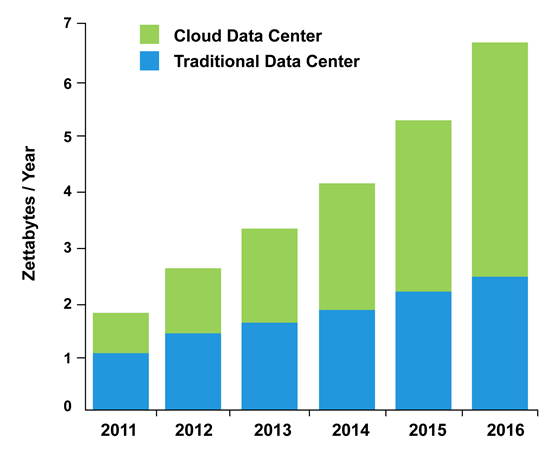
\includegraphics[width=5in]{Resources//1.png}
\caption{Image source: http://thirdmillenniumtimes.com/ \cite{ThirdMilleniumTimesInternetIsStillGrowingFast}, Web page representation of image acknowledges data source as Cisco Global Cloud Index: Forecast and Methodology, 2012–2017 \cite{CiscoGlobalCloudIndex:ForecastAndMethodology}.}
\label{fig:ThirdMilleniumTimesBarGraph}
\end{figure}

Naturally, this increase has lead \gls{data centre}s to become major users of electricity, with ever increasing demand for better processors and more storage in the systems located therein. Koomey shows that of all electricity used globally in 2005, 1\% of it was used in the operation of \gls{data centre}s, which is an increase from the 2000 figure of 0.5\% \cite{KoomeyGrowthInDataCenterElectricityUse}.

This presents a conundrum: cloud-computing and other \gls{data centre} dependant technologies are becoming ever more popular, which is driving \gls{data centre}s to become less sustainable in terms of general energy consumption. \textcolor{red}{Therefore, it is necessary to take steps towards bringing \gls{data centre}s in line with energy efficiency goals.[UPDATE THIS WITH TEXT FROM THE PRESENTATION}

\subsection{Goals of this Project}
\label{sec:Background:GoalsOfThisProject}
This project aims to produce a game in which the user must outfit a data centre. This will follow the format of being a strategy game, which will consider the following principles in its design:

\begin{itemize}

\item In order to present this game to as wide an audience as possible it will be developed as an internet-browser based game \textcolor{red}{, and, upon completion of this aspect of it, may be ported to mobile gaming platforms such as Android and ios.}

\item This game will require users to take account of energy-efficiency, cost-effectiveness and operational efficiency of their data centre while they design it.

\item In order to fulfil these goals, players of the game will require users to select components for their \gls{data centre} as they set it up, each of which will have an impact on an overall aggregate score for the \gls{data centre}, which will be derived using the three criteria mentioned above.

\end{itemize}

\subsubsection{Justification}
\label{sec:ProjectGoal:Justification}
The justifications for this project are twofold:

\begin{enumerate}
\item To bring awareness of cloud-computing environmental concerns to Internet users, doing so by providing the information in an accessible format.

\item To provide a means of demonstrating what is required to design a data centre in a format accessible to general users.
\end{enumerate}

\subsection{Study Plan}
\label{sec:Background:StudyPlan}
This study will consist of the following elements in the following sequence:

\begin{enumerate}
\item A literature review of real world concepts and technologies relevant to this project. These will include the following:
\begin{itemize}
\item Studies into the environmental effect of \gls{data centre}s, seeking to ascertain the chief concerns in this area so that appropriate ways of modelling them in the game can be devised.

\item Studies into the energy efficiency and cost effectiveness of devices and elements of \gls{data centre}s, such as Central Processing Units (CPUs), cooling systems, storage systems, memory systems etc.

\item Studies into the application of Artificial-Intelligence in strategy games such as Sim-City, Civilization and The Sims. \textcolor{red}{CITE THESE GAME NAMES.}

\item Studies of browser-games developed using JavaScript.
\end{itemize}

\item With the information gathered from section \ref{sec:ACriticalReviewOfReleventScientificAndEngineeringLiturature}, a three-part game platform will be developed. These parts are as follows:
\begin{enumerate}
\item A database of elements to be used in game, representing real world components and elements used within the \gls{data centre}. An example would be a \textcolor{red}{CPU type[BAD EXAMPLE, GO WITH SERVER AND UP]}, which would itself have attributes such as optimal operating temperature in degrees Celsius, speed in gigahertz, cost in US dollars and energy consumption in kilowatt-hours. Another example would be a particular cooling system, which would have attributes such as temperature reduction in degrees Celsius and energy consumption in kilowatt-hours.

\item A database of logic and rules to be checked in game-play. Such rules could include the following:
\begin{itemize}
\item \textcolor{red}{If a CPU has a set temperature at which it overheats, and lacks an adequate cooling system to prevent it exceeding this temperature, a rule should be included to say that  the CPU will malfunction. Other rules would link into this, for example, the loss of this CPU could lead the overall operating speed of the data-center to fall, which could lead the reputation of the data-center with customers to fall also.[BAD EXAMPLE: GO WITH SERVER AND UP]}

\item Operating more processors at night time when it is cooler could lead to lower costs due to lower temperature, but may lead to a drop in the \gls{data centre}'s reputation with customers due to inconsistent speeds.
\end{itemize}

\item A basic test program, allowing the user to input commands such as to use a certain type of CPU, seeing how the logic-engine part of the program
responds under different conditions.
\end{enumerate}

\textcolor{red}{Specifically, the test program, and later the game platform itself will be written in JavaScript, allowing dynamic user interaction. This will be embedded in a page utilising CSS and HTML5 coding.}

\item 
This test-program will be tested under differing conditions. This will serve as a white-box test of the component database and the logic engine elements of the application.

\item An interface between the database and logic-engine components of the application will be developed, along with a Graphical User Interface (GUI).

\item The program will undergo a final stage of testing.
\end{enumerate}